\subsection{Graph construction}
Using the geographic information of the roads and buildings, a graph
is constructed for each neighborhood, using the \url{igraph} module in \url{Python}. This graph
connects all buildings to each other over the road network. First, using the information about the
roads and buildings the sets of nodes and edges need to be defined. An edge is a line that connects
two edges to each other. Extracting the edges that connect the road network is straightforward,
since all roads already have an ordered list of nodes defined. The subsequent nodes simply need to
be stored as pairs, and all edges are defined.

When the road network is defined as a set of nodes and edges, the next step is to connect the buildings
to the road network. This needs to be implemented manually, since no data is stored in OpenStreetMap
about to which road the buildings belong. This algorithm needs to be very efficient, since many
buildings are added in each area. An R-tree can be used to accomplish this efficiency.
An R-tree is a dynamic index structure that is able to retrieve data items quickly according to
their spatial locations \citep{guttman1984r}. Listing \ref{lst:python-edges} displays the algorithm
used to make the edges that connect the buildings to the road network. For each building node,
the closest point on the closest road is found, using the shapely implementation of the R-tree,
\pythoninline{STRtree}. Then, if this point is not an already existing node, a new virtual node is added,
which splits this existing edge in two parts. The road is reconnected with the new node in between.
Finally, the building is connected to this new node.

In order to find the shortest path in terms of real distance, and to calculate the length of the
TSP path, a 'weight' needs to be added. This weight represents the length of this edge in meters.
The equirectangular approximation is used to calculate these weights. This approximation is very
efficient, but only works when the points the distance is calculated between is small enough such
that the rounding of the earth does not have a significant effect on the true distance.
The nodes are all close enough together, so the effect of the
rounding of earth's surface is negligible. Let $A$ and $B$ be two nodes,
and $(\varphi_A,\theta_A)$, $(\varphi_B,\theta_B)$ be their coordinates, in \url{radians}. Let $R=6,371,000$ meters,
Earth's radius. Then the distance between these nodes (the weight of the edge connecting them),
using the equirectangular approximation is:
\begin{align}
	\label{eq:equirectangluar_approx}
	d(A,B)               & =R\sqrt{\varphi^2+\theta^2},                             \\
	\text{where }\varphi & =(\varphi_B-\varphi_A)\cos{\frac{\theta_A+\theta_B}{2}}, \\
	\text{and }\theta    & =\theta_B-\theta_A.
\end{align}

Using the \url{folium} module in \url{Python}, such a graph can be visualized on a geographic map.
One of such visualizations is provided in figure \ref{fig:overtoomse_sluis}. All maps like this one,
for the areas in this analysis can be viewed and interacted with via this
\href{https://koenstevens.nl/projects/BSc_thesis/maps/}{\url{webpage}}.
\begin{figure}[H]
	\caption{Visualization of the graph, for the Overtoomse Sluis quarter in Amsterdam.}
	\label{fig:overtoomse_sluis}
	\includegraphics[width=\textwidth]{Pictures/Overtoomse_Sluis_roads.png}
\end{figure}

\subsection{Extracting features}
One of the predictors of the TSP path length, is the area of the neighborhood the locations are drawn from.
The OSM data provides the area of the polygons, but this value can not be used to predict TSP path length effectively.
This value significantly overestimates the correct value for $A$.
When there are things like parks, lakes, or large buildings like a stadium inside the quarter, then in that part of the
area, there are no delivery locations. Consequently, this area should not be included in the area calculation.
To account for this problem, alpha shapes are used to calculate $A$. Alpha shapes are generalizations of the convex hull,
they capture the shape of a point set \citep{akkiraju1995alpha}. Figure \ref{fig:Beijum} displays the map of the Beijum
quarter in Groningen with the alpha shape for its addresses, as it was used for calculating the area.
It can be seen that using this method, large areas without buildings, such as the greenspace in the middle is being left
out, as desired.
% \begin{figure}[H]
% 	\centering
% 	\begin{subfigure}[b]{0.45\textwidth}
% 		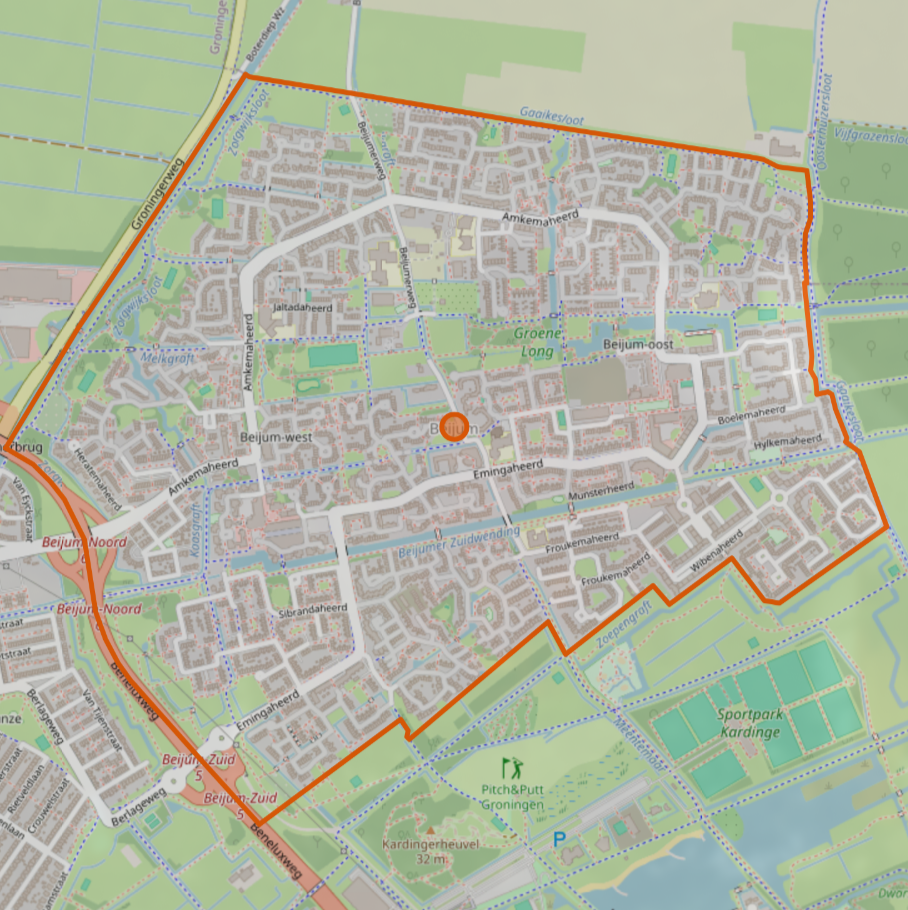
\includegraphics[width=\textwidth]{Pictures/Beijum_quarter.png}
% 		\caption{Beijum on the map}
% 		\label{fig:Beijummap}
% 	\end{subfigure}
% 	\hfill
% 	\begin{subfigure}[b]{0.45\textwidth}
% 		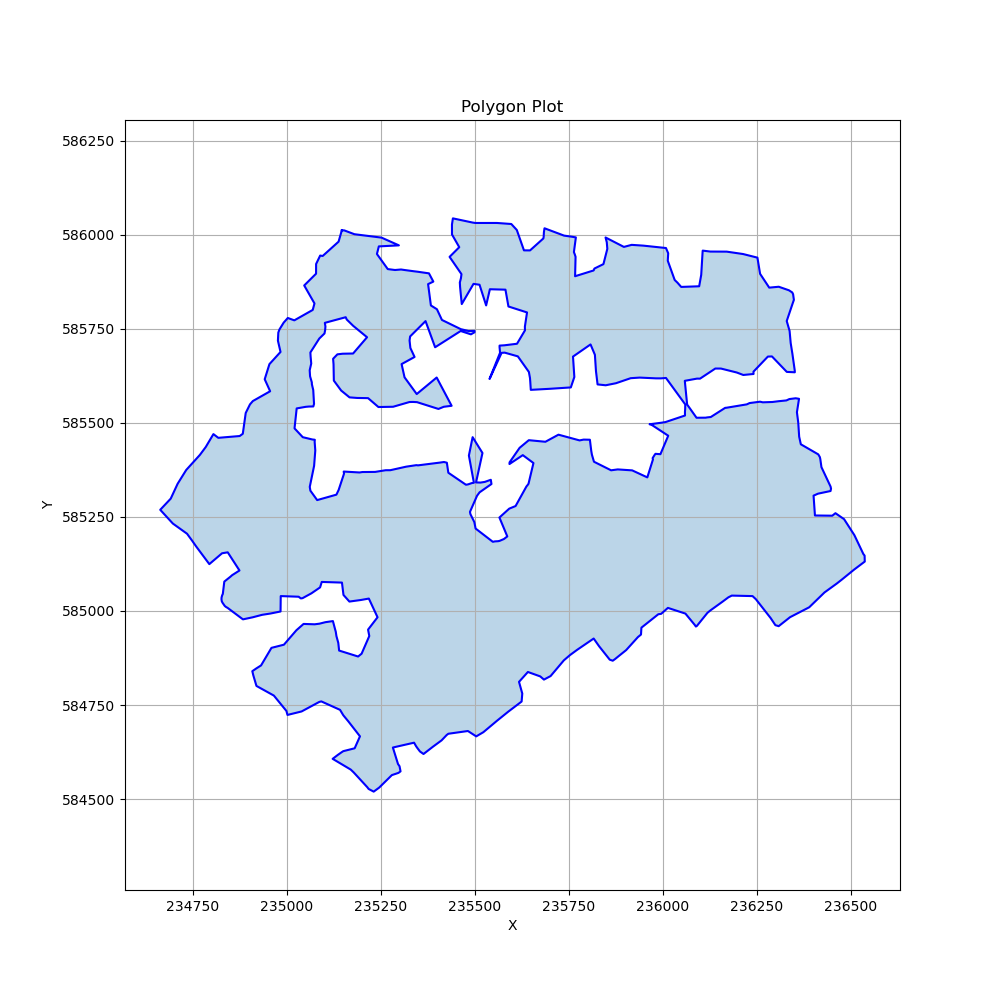
\includegraphics[width=\textwidth]{Pictures/hull_beijum.png}
% 		\caption{The alpha shape for the addresses}
% 		\label{fig:AlphaBeijum}
% 	\end{subfigure}
% 	\caption{The map of the Beijum quarter in Groningen, with the alpha shape around its addresses.}
% 	\label{fig:Beijum}
% \end{figure}
\begin{figure}[H]
	\centering
	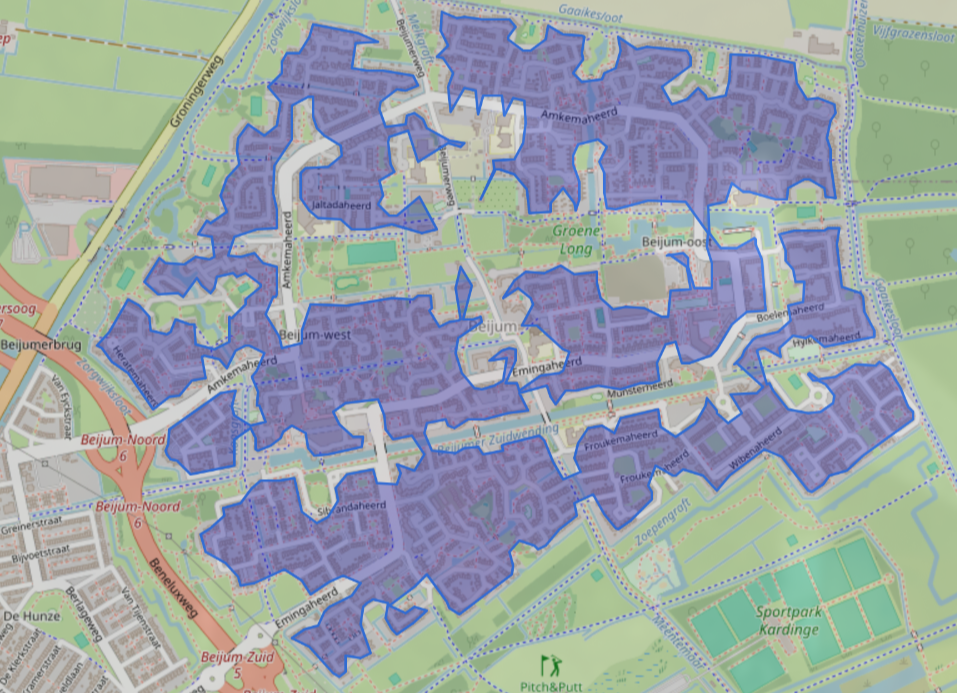
\includegraphics[width=\textwidth]{Pictures/better_hull_beijum.png}
	\caption{The map of the Beijum quarter in Groningen, with the alpha shape around its addresses.}
	\label{fig:Beijum}
\end{figure}

While the area of a neighborhood is an important predictor, it is only one of many features considered in this analysis.
To train a supervised learning model that predicts the TSP path length based on neighborhood characteristics, a comprehensive set
of features needs to be extracted.

In total, approximately 80 features are gathered for each neighborhood. These features describe various aspects of the built environment, infrastructure,
and spatial distribution of delivery locations. They fall broadly into the following categories:

\begin{itemize}
	\item \textbf{Geographic features:} the area of the alpha shape around all postcodes, characteristics such as how much water or how many parks,
	      and land use (i.e. residential or commercial).
	\item \textbf{Road network metrics:} Percentage of roads that are one-way, total length of road network divided by the area of the alpha shape.
	\item \textbf{Graph-technical properties}: average edge length, average path length between all nodes in the graph, clustering properties.
\end{itemize}

The clustering properties might be particularly interesting. The assumption in the BHH formula that the locations are uniformly distributed across the area is
the one the setup in this research violates. Using these properties in the supervised learning model might lead to more accurate predictions. The metrics that were
used for this are:
\begin{itemize}
	\item The number of communities according to the \url{infomap} method\\ \citep{rosvall2008maps}. This might provide information about clustering of
	      addresses on the scale of sub-neighborhoods inside a quarter with space in between.
	\item The mean, max, and variance of the degree of the nodes. The degree of a node is the number of edges are connected to it.
	      For example, when there is a large apartment building, often times all these different addresses connect to the exact same spot on a road.
	      Then, this road node has a very large degree, sometimes more than 100. The mean, variance and maximum of this number all might provide some information
	      about this local clustering.
	\item The diameter of the graph: the maximum shortest-path distance between any two nodes.
	\item The radius of the graph: the minimum eccentricity of any node, where eccentricity is the maximum shortest-path distance to any other node.
\end{itemize}
